
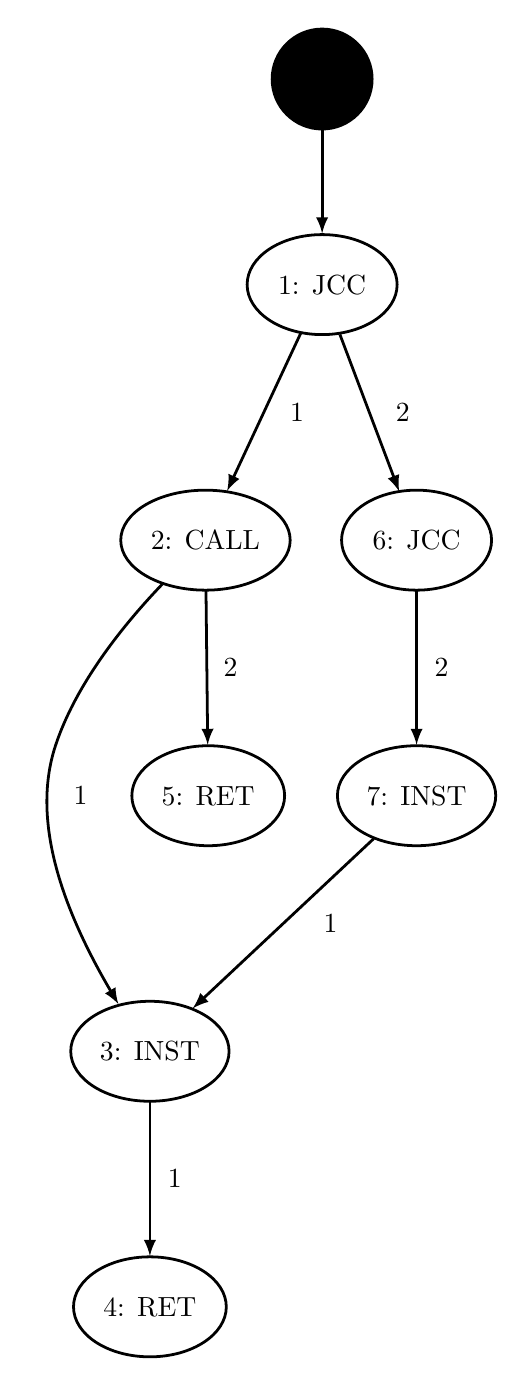
\begin{tikzpicture}[>=latex,line join=bevel,]
  \pgfsetlinewidth{1bp}
%%
\pgfsetcolor{black}
  % Edge: 2 -> 3
  \draw [->] (41.758bp,278.18bp) .. controls (28.646bp,264.51bp) and (10.832bp,242.91bp)  .. (3.2809bp,220.0bp) .. controls (-6.2226bp,191.17bp) and (7.8073bp,157.83bp)  .. (25.961bp,126.94bp);
  \definecolor{strokecol}{rgb}{0.0,0.0,0.0};
  \pgfsetstrokecolor{strokecol}
  \draw (12.281bp,202.0bp) node {1};
  % Edge: 6 -> 7
  \draw [->] (133.28bp,275.65bp) .. controls (133.28bp,262.82bp) and (133.28bp,245.11bp)  .. (133.28bp,220.3bp);
  \draw (142.28bp,248.0bp) node {2};
  % Edge: 1 -> 6
  \draw [->] (105.68bp,368.07bp) .. controls (110.69bp,354.79bp) and (117.76bp,336.07bp)  .. (127.03bp,311.55bp);
  \draw (128.28bp,340.0bp) node {2};
  % Edge: 7 -> 3
  \draw [->] (117.86bp,186.54bp) .. controls (102.32bp,171.98bp) and (78.166bp,149.33bp)  .. (52.667bp,125.42bp);
  \draw (102.28bp,156.0bp) node {1};
  % Edge: 1 -> 2
  \draw [->] (91.577bp,368.49bp) .. controls (85.4bp,355.25bp) and (76.614bp,336.43bp)  .. (65.078bp,311.71bp);
  \draw (90.281bp,340.0bp) node {1};
  % Edge: 0 -> 1
  \draw [->] (99.281bp,441.94bp) .. controls (99.281bp,433.81bp) and (99.281bp,423.88bp)  .. (99.281bp,404.44bp);
  % Edge: 2 -> 5
  \draw [->] (57.474bp,275.65bp) .. controls (57.616bp,262.82bp) and (57.813bp,245.11bp)  .. (58.089bp,220.3bp);
  \draw (66.281bp,248.0bp) node {2};
  % Edge: 3 -> 4
  \draw [->] (37.281bp,91.647bp) .. controls (37.281bp,78.823bp) and (37.281bp,61.108bp)  .. (37.281bp,36.3bp);
  \draw (46.281bp,64.0bp) node {1};
  % Node: 1
\begin{scope}
  \definecolor{strokecol}{rgb}{0.0,0.0,0.0};
  \pgfsetstrokecolor{strokecol}
  \draw (99.28bp,386.0bp) ellipse (27.0bp and 18.0bp);
  \draw (99.281bp,386.0bp) node {1: JCC};
\end{scope}
  % Node: 0
\begin{scope}
  \definecolor{strokecol}{rgb}{0.0,0.0,0.0};
  \pgfsetstrokecolor{strokecol}
  \definecolor{fillcol}{rgb}{0.0,0.0,0.0};
  \pgfsetfillcolor{fillcol}
  \filldraw [opacity=1] (99.28bp,460.0bp) ellipse (18.0bp and 18.0bp);
\end{scope}
  % Node: 3
\begin{scope}
  \definecolor{strokecol}{rgb}{0.0,0.0,0.0};
  \pgfsetstrokecolor{strokecol}
  \draw (37.28bp,110.0bp) ellipse (28.5bp and 18.0bp);
  \draw (37.281bp,110.0bp) node {3: INST};
\end{scope}
  % Node: 2
\begin{scope}
  \definecolor{strokecol}{rgb}{0.0,0.0,0.0};
  \pgfsetstrokecolor{strokecol}
  \draw (57.28bp,294.0bp) ellipse (30.5bp and 18.0bp);
  \draw (57.281bp,294.0bp) node {2: CALL};
\end{scope}
  % Node: 5
\begin{scope}
  \definecolor{strokecol}{rgb}{0.0,0.0,0.0};
  \pgfsetstrokecolor{strokecol}
  \draw (58.28bp,202.0bp) ellipse (27.5bp and 18.0bp);
  \draw (58.281bp,202.0bp) node {5: RET};
\end{scope}
  % Node: 4
\begin{scope}
  \definecolor{strokecol}{rgb}{0.0,0.0,0.0};
  \pgfsetstrokecolor{strokecol}
  \draw (37.28bp,18.0bp) ellipse (27.5bp and 18.0bp);
  \draw (37.281bp,18.0bp) node {4: RET};
\end{scope}
  % Node: 7
\begin{scope}
  \definecolor{strokecol}{rgb}{0.0,0.0,0.0};
  \pgfsetstrokecolor{strokecol}
  \draw (133.28bp,202.0bp) ellipse (28.5bp and 18.0bp);
  \draw (133.28bp,202.0bp) node {7: INST};
\end{scope}
  % Node: 6
\begin{scope}
  \definecolor{strokecol}{rgb}{0.0,0.0,0.0};
  \pgfsetstrokecolor{strokecol}
  \draw (133.28bp,294.0bp) ellipse (27.0bp and 18.0bp);
  \draw (133.28bp,294.0bp) node {6: JCC};
\end{scope}
%
\end{tikzpicture}

